% Created by Oscar de Felice
% Last update: September, 4 2020 by Oscar de Felice

% Authors: Oscar de Felice
% Please do not make changes to the preamble until after the solid line of %s.

\documentclass[10pt]{article}
\usepackage[explicit]{titlesec}
\setlength{\parindent}{0pt}
\setlength{\parskip}{1em}
\usepackage{hyphenat}
\usepackage{ragged2e}
\RaggedRight

% These commands change the font.
% If you do not have Garamond on your computer, you will need to install it.
\usepackage{garamondx}
\usepackage[T1]{fontenc}
\usepackage[utf8]{inputenc}
\usepackage{amsmath, amsthm}
\usepackage{graphicx}

% This adjusts the underline to be in keeping with word processors.
\usepackage{soul}
\setul{.6pt}{.4pt}


% The following sets margins to 1 in. on top and bottom and .75 in on left
% and right, and remove page numbers.
\usepackage{geometry}
\geometry{vmargin={1in,1in}, hmargin={.75in, .75in}}
\usepackage{fancyhdr}
\pagestyle{fancy}
\pagenumbering{gobble}
\renewcommand{\headrulewidth}{0.0pt}
\renewcommand{\footrulewidth}{0.0pt}

% These Commands create the label style for tables, figures and equations.
\usepackage[labelfont={footnotesize,bf} , textfont=footnotesize]{caption}
\captionsetup{labelformat=simple, labelsep=period}
\newcommand\num{\addtocounter{equation}{1}\tag{\theequation}}
\renewcommand{\theequation}{\arabic{equation}}
\makeatletter
\renewcommand\tagform@[1]{\maketag@@@ {\ignorespaces {\footnotesize{\textbf{Equation}}} #1.\unskip \@@italiccorr }}
\makeatother
\setlength{\intextsep}{10pt}
\setlength{\abovecaptionskip}{2pt}
\setlength{\belowcaptionskip}{-10pt}

\renewcommand{\textfraction}{0.10}
\renewcommand{\topfraction}{0.85}
\renewcommand{\bottomfraction}{0.85}
\renewcommand{\floatpagefraction}{0.90}

% These commands set the paragraph and line spacing
\titleformat{\section}
  {\normalfont}{\thesection}{1em}{\MakeUppercase{\textbf{#1}}}
\titlespacing\section{0pt}{0pt}{-10pt}
\titleformat{\subsection}
  {\normalfont}{\thesubsection}{1em}{\textit{#1}}
\titlespacing\subsection{0pt}{0pt}{-8pt}
\renewcommand{\baselinestretch}{1.15}

% This designs the title display style for the maketitle command
\makeatletter
\newcommand\sixteen{\@setfontsize\sixteen{16pt}{6}}
\renewcommand{\maketitle}{\bgroup\setlength{\parindent}{0pt}
\begin{flushleft}
\vspace{-.375in}
\sixteen\bfseries \@title
\medskip
\end{flushleft}
\textit{\@author}
\egroup}
\makeatother

% This styles the bibliography and citations.
%\usepackage[biblabel]{cite}
\usepackage[sort&compress]{natbib}
\setlength\bibindent{2em}
\makeatletter
\renewcommand\@biblabel[1]{\textbf{#1.}\hfill}
\makeatother
\renewcommand{\citenumfont}[1]{\textbf{#1}}
\bibpunct{}{}{,~}{s}{,}{,}
\setlength{\bibsep}{0pt plus 0.3ex}




%%%%%%%%%%%%%%%%%%%%%%%%%%%%%%%%%%%%%%%%%%%%%%%%%

% Authors: Add additional packages and new commands here.
% Limit your use of new commands and special formatting.

% Place your title below. Use Title Capitalization.
\title{Moore's Law}

% Add author information below.
% Communicating author is indicated by an asterisk, the affiliation is shown
% by superscripted lower case letter if several affiliations need to be noted.
\author{
Oscar de Felice$^{a}$\\ \medskip \bigskip
$^{a}$LaJavaness, 19 rue Martel, 75010 Paris \\ \medskip \bigskip
}

\pagestyle{empty}
\begin{document}

% Makes the title and author information appear.
\vspace*{.01 in}
\maketitle
\vspace{.12 in}

% Abstracts are required.
\section*{Moore's Law}
Moore's law is the observation that the number of transistors in a dense integrated circuit doubles about every two years.
This law -- which is more an observation and projection of a historical trend -- is named after George Moore, the co-founder of Fairchild Semiconductor and CEO and co-founder of Intel, who in 1965 posited a doubling every year in the number of components per integrated circuit, and projected this rate of growth would continue for at least another decade.
As said, rather than a law of physics, it is an empirical relationship linked to gains from experience in production.

% Keywords are required.
\section*{keywords}
Moore's law; Transistors; Integrated Circuit; Computer

\vspace{.12 in}

% Start the main part of the manuscript here.
% Comment out section headings if inappropriate to your discipline.
% If you add additional section or subsection headings, use an asterisk * to avoid numbering.

\section*{Introduction}
Moore's law is the observation that the number of transistors in a dense integrated circuit doubles about every two years.
This law -- which is more an observation and projection of a historical trend -- is named after George Moore, the co-founder of Fairchild Semiconductor and CEO and co-founder of Intel, who in 1965 posited a doubling every year in the number of components per integrated circuit, and projected this rate of growth would continue for at least another decade.
In 1975, looking forward to the next decade, he revised the forecast to doubling every two years.
As said, rather than a law of physics, it is an empirical relationship linked to gains from experience in production.

\section*{Limits}
Although the rate held steady from 1975 until around 2012, the rate was faster during the first decade.
In general, it is not logically sound to extrapolate from the historical growth rate into the indefinite future.
For instance, the 2010 update to the \emph{International Technology Roadmap for Semiconductors} predicted that growth would slow around 2013, and in 2015 the same Gordon Moore foresaw that the rate of progress would reach saturation:

\begin{displayquote}
  I see Moore's law dying here in the next decade or so.
\end{displayquote}

\subsection*{Reason of the end of Moore's law}
One can list the several reasons at the root of the end of Moore's law:

\begin{enumerate}
\item As transistors increase, power demand increases, which
increases heat.
\item Smaller transistors switch faster, increasing power demand.
\item Exponential increase in density would lead to
exponential increase in speed
\item Transistor’s need a minimum voltage to switch, and
voltage reduction has lower limits due to noise.
\item Dynamic power consumption is reduced by voltage
scaling.
\item Voltage scaling does not prevent power leakage.
\end{enumerate}

% Add an image
\begin{figure}[ht!]
\centering
  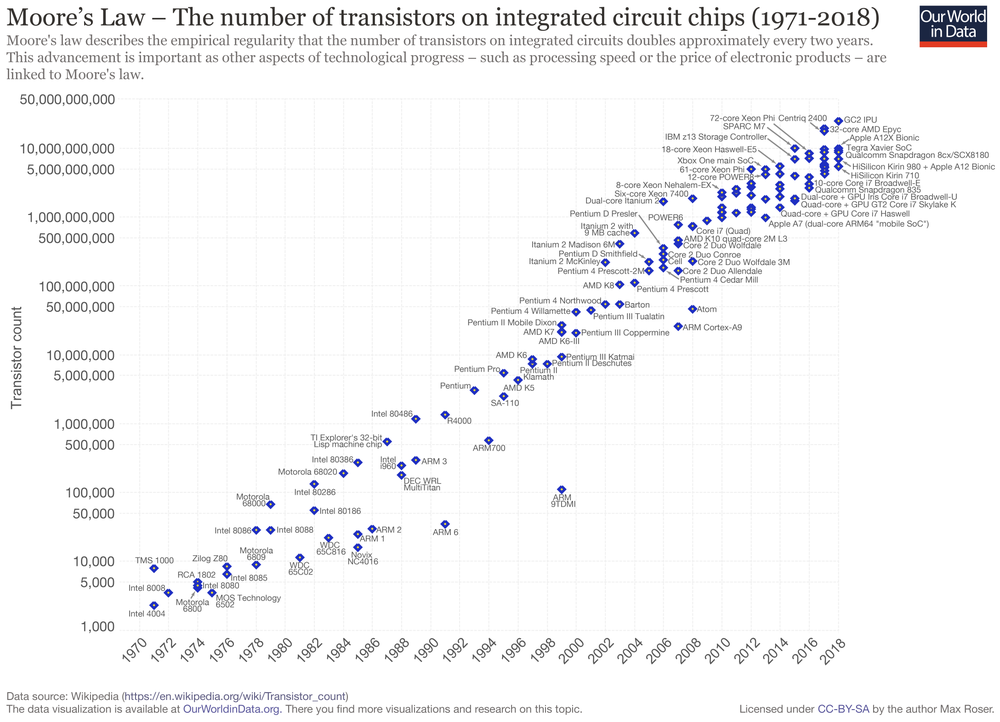
\includegraphics[width=0.5\textwidth]{Images/Moore's_Law_Transistor_Count.png}
\caption{A semi-log plot of transistor counts for microprocessors against dates of introduction, nearly doubling every two years.}\label{Mooreslaw}
\end{figure}

\section*{conclusions}
As said in the beginning, Moore's law is not a physical law.
It was just an extrapolation of a trend, only true in a very specific moment of time.
A good programmer should not base the good performances of its softwares only on hardware capacity.

\end{document}
